\section{自适应分段逼近}
\label{sec:fapprox-adaptive}

第~\ref{sec:fapprox-fixed-grid}节的固定网格在看到目标之前就选定了分点，误差由目标在最差单元上的局部正则性决定。若目标只在少数地方变化剧烈，更合理的做法是在那里多放分点，在平缓处少放。上一节只调整“留哪几个坐标”，这里连坐标轴本身也按目标调整：分点就是把长向量的下标切成几段的位置。

本节把预算固定为区间个数$N$，允许分点随目标移动，在一致范数下比较固定网格与自适应分割，并区分三个问题：最佳分割是否存在，它的误差有多大，以及怎样找到一个好的分割。

\paragraph{候选集合与局部误差}
在$[0,1]$上，令$\mathcal S_N$为全体至多$N$段的分段常数函数：存在$0=x_0\leq x_1\leq\cdots\leq x_N=1$，函数在每个$[x_{i-1},x_i)$上为常数，最后一段含右端点。分点是候选的一部分，所以$\mathcal S_N$不是线性空间，相应的逼近称为\term{自适应分段逼近}（adaptive piecewise approximation）。

分割固定后，每段上的最佳常数由式~\eqref{eq:fapprox-best-constant}给出：在$I=[a,b]$上，局部误差是振幅的一半，记为$\frac12\operatorname{osc}(f,I)$，其中$\operatorname{osc}(f,I)=\max_If-\min_If$。所以对连续的$f$，
\begin{equation}
 E(f,\mathcal S_N)_\infty=\frac12\inf_{0=x_0\leq\cdots\leq x_N=1}\ \max_{1\leq i\leq N}\operatorname{osc}\bigl(f,[x_{i-1},x_i]\bigr).
 \label{eq:fapprox-adaptive-error}
\end{equation}
寻找最佳逼近化成了一个只关于分点的问题：让最大的局部振幅尽可能小。

\paragraph{平方根函数的比较}
以$f(x)=\sqrt x$为例。它在$[0,1]$上连续递增，但在原点附近导数无界，不是Lipschitz的。等距网格$x_i=i/N$上，单元$[x_{i-1},x_i]$的振幅是
\[
 \sqrt{\frac iN}-\sqrt{\frac{i-1}N},
\]
随$i$递减，最大的是第一个单元的$\sqrt{1/N}$。所以固定网格的误差为
\[
 \frac1{2\sqrt N}.
\]

若改取$x_i=(i/N)^2$，每个单元的振幅都是
\[
 \sqrt{x_i}-\sqrt{x_{i-1}}=\frac1N ,
\]
误差为$1/(2N)$。$N=100$时，前者为$0.05$，后者为$0.005$。分点向原点聚集，把局部误差平均分配到各个单元。图~\ref{fig:fapprox-adaptive}(a)(b)画出$N=6$的两种分割。

这个分割还是最优的。任一分割的各段振幅之和为
\[
 \sum_i\bigl(\sqrt{x_i}-\sqrt{x_{i-1}}\bigr)=1 ,
\]
$N$个数之和为$1$，最大者不小于$1/N$。所以$E(\sqrt{\cdot},\mathcal S_N)_\infty=1/(2N)$，自适应分段把速率从$N^{-1/2}$提高到$N^{-1}$，而固定网格要达到同样的速率需要目标是Lipschitz的。

\begin{BookInlineFigure}
  \centering
  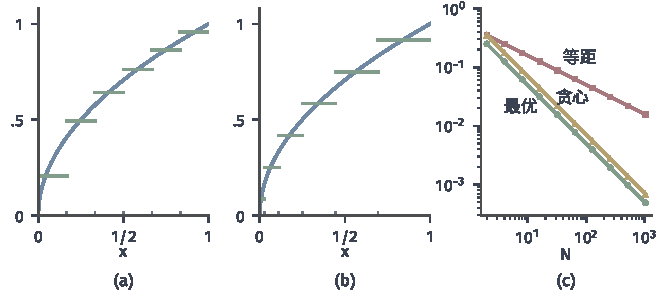
\includegraphics[width=112mm]{figures/04-spaces-measures-and-geometry/03-function-spaces/matplotlib/fapprox-adaptive/figure.pdf}
  \caption{$\sqrt x$的分段常数逼近，每段取最佳常数（绿），下方刻线为分点。(a)$N=6$的等距分割，误差集中在第一段。(b)$N=6$的分割$x_i=(i/6)^2$，每段振幅相同。(c)一致误差随段数$N$的变化，双对数坐标：等距为$1/(2\sqrt N)$，最优为$1/(2N)$，二进贪心细分的误差约为最优的$\sqrt2$倍。}
  \label{fig:fapprox-adaptive}
\end{BookInlineFigure}

\paragraph{单调函数的误差界}
平方根例子中用到的只是单调性，并不需要可微。把振幅之和等于总变化量的论证写成一般形式，就得到下面的结论。

\begin{theorem}[单调函数的自适应分段误差]
\label{thm:fapprox-monotone}
设$f$在$[a,b]$上连续且单调，$V=\lvert f(b)-f(a)\rvert$。则
\begin{equation}
 E(f,\mathcal S_N)_\infty=\frac V{2N},
 \label{eq:fapprox-monotone}
\end{equation}
并且存在达到这一误差的分割。
\end{theorem}

\begin{proof}
不妨设$f$不减。对任一分割，各段振幅为$f(x_i)-f(x_{i-1})$，其和为$V$，最大者不小于$V/N$，所以误差不小于$V/(2N)$。

反过来，令$x_0=a$，对$i=1,\ldots,N$取
\[
 x_i=\min\Bigl\{x\in[a,b]:\ f(x)=f(a)+\frac{iV}N\Bigr\}.
\]
由介值定理这样的点存在，由连续性最小值能取到，水平递增时这些点不减。$x_N\leq b$，把最后一个分点改成$b$，$f$在多出的一段上恒为$f(b)$，不改变取值范围。

在$[x_{i-1},x_i]$上，$f$的取值落在$f(a)+(i-1)V/N$与$f(a)+iV/N$之间，振幅不超过$V/N$。由式~\eqref{eq:fapprox-adaptive-error}，误差不超过$V/(2N)$。
\end{proof}

定理把误差与总变化量$V$联系起来，而不是与导数或连续模联系。固定网格的误差由$\omega_f(h)$控制，要求处处都不能变化太快；自适应分割只要求变化的总量有限，变化集中在哪里都可以。在同一预算和同一误差范数下，两种候选集合对目标正则性的要求不同。

\paragraph{最佳分割的存在}
对一般的连续函数，最佳分割同样存在，但通常没有显式公式。分点向量$(x_1,\ldots,x_{N-1})$在紧集$\{0\leq x_1\leq\cdots\leq x_{N-1}\leq1\}$中变化。由$f$一致连续，$\operatorname{osc}(f,[a,b])$是$(a,b)$的连续函数：端点移动不超过$\eta$时，最大值与最小值各自至多改变$\omega_f(\eta)$。

所以最大局部振幅是分点的连续函数，在紧集上取到最小值。允许相邻分点重合，相当于允许少于$N$段，并不改变$\mathcal S_N$。这一论证和第~\ref{sec:fapprox-fixed-space}节的存在定理一样靠紧性，只是紧的集合从有限维子空间中的闭球换成了分点的单纯形。

存在性与误差界是两回事。存在性论证没有说明最佳误差有多大，也没有给出找到最佳分割的方法；单调函数的定理给出了误差的精确值，构造却依赖于知道$f$的水平集位置。

\paragraph{贪心细分}
实际中常用的是一种简单的算法：从整个区间出发，每一步找出局部误差最大的单元，把它从中点一分为二，直到用完$N$个单元。每步只需计算新产生的两个单元的振幅，分点都落在二进点上。

用$\sqrt x$跑前几步。第一步把$[0,1]$对半切，两段的振幅是
\[
 \operatorname{osc}\bigl(\sqrt{\cdot},[0,\tfrac12]\bigr)=0.7071,\qquad
 \operatorname{osc}\bigl(\sqrt{\cdot},[\tfrac12,1]\bigr)=0.2929 .
\]
第二步切振幅最大的$[0,\frac12]$，得到$[0,\frac14]$的振幅$0.5$和$[\frac14,\frac12]$的振幅$0.2071$。第三步切$[0,\frac14]$，得到振幅$0.3536$和$0.1464$。

这时四个单元从左到右的振幅是
\[
 0.3536,\quad 0.1464,\quad 0.2071,\quad 0.2929 .
\]
最大误差是$0.3536/2=0.1768$，而$N=4$的最优误差是$1/8=0.125$。贪心细分总是先切靠近原点的单元，却只能对半切，各单元的振幅不能像最优分割那样恰好相等。

表~\ref{tab:fapprox-greedy}列出了几种$N$的结果。这个例子中贪心误差始终是最优误差的约$\sqrt2$倍，也就是说，它达到了与最优分割相同的速率$N^{-1}$，只损失一个常数。这是对$\sqrt x$的计算观察，不是一般定理；贪心细分与最佳误差的比较需要针对目标类另作分析。

\begin{BookInlineTable}
  \centering
  \caption{$\sqrt x$的分段常数逼近的一致误差}
  \label{tab:fapprox-greedy}
  \begin{tabular}{rlll}
    \toprule
    $N$ & 等距$1/(2\sqrt N)$ & 贪心细分 & 最优$1/(2N)$ \\
    \midrule
    $4$ & $0.25$ & $0.1768$ & $0.125$ \\
    $16$ & $0.125$ & $0.0442$ & $0.0313$ \\
    $64$ & $0.0625$ & $0.0110$ & $0.0078$ \\
    $1024$ & $0.0156$ & $0.00069$ & $0.00049$ \\
    \bottomrule
  \end{tabular}
\end{BookInlineTable}

二进的贪心细分与上一节的Haar展开密切相关：在二进区间上保留或舍去细分，相当于在Haar展开中保留或舍去对应的细节系数。哪些函数能被这样的自适应表示以给定速率逼近，可以用函数在不同尺度上的局部变化来刻画，这正是第~\ref{chap:besov-spaces}章研究的问题。
